\begin{flushright} {\tiny {\color{gray} \tt storage.tex}} \end{flushright}
%~~~~~~~~~~~~~~~~~~~~~~~~~~~~~~~~~~~~~~~~~~~~~~~~~~~~~~~~~~~~~~~~~~~~~~~~~~~~~~~~~~~~~~~~~~~~~~~~~~

The FE matrix\footnote{what follows also applied to matrices 
obtained by means of the FD method} (or the blocks which compose it) 
is the result of the assembly process of all elemental matrices. 
Its size can become quite large when the resolution is being increased (from thousands
of lines/columns to tens of millions, if not even more).

One important property of the matrix is its sparsity. Typically musc {\it much} less than 1\% of the 
matrix terms is not zero and this means that the matrix storage can and {\it should} be optimised. 
Clever storage formats were designed early on since the amount of RAM memory in computers
was the limiting factor 3 or 4 decades ago \cite{saad}.

There are several standard formats\footnote{\url{https://en.wikipedia.org/wiki/Sparse_matrix}}, e.g.:
\begin{itemize}
\item compressed sparse row format (CSR) \index{general}{CSR} \index{general}{Compressed Sparse Row}
\item compressed sparse column format (CSC) \index{general}{CSC} \index{general}{Compressed Sparse Column}
\item the Coordinate Format (COO)
\item Skyline Storage Format
\end{itemize}

I focus on  the CSR format in what follows since it is the most common format 
and it is the one used in \elefant and in almost all code of FieldStone. 
In the following sections I look at typical cases in 2d and 3d.

%..............................................................................
\subsection{2d domain - $Q_1$ - One degree of freedom per node}

Let us consider again the  $3\times2$ element grid which counts 12 nodes.

\begin{center}
\begin{flushright} {\tiny {\color{gray} (tikz\_3x2.tex)}} \end{flushright}
%~~~~~~~~~~~~~~~~~~~~~~~~~~~~~~~~~~~~~~~~~~~~~~~~~~~~~~~~~~~~~~~~~~~~~~~~~~~~~~~~~~~~~~~~~~~~~~~~~~

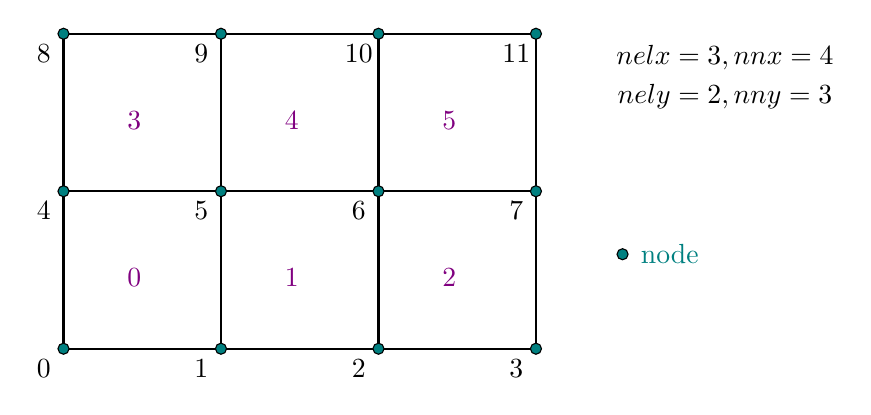
\begin{tikzpicture}
%\draw[step=0.5cm,gray,very thin] (0,0) grid (9,5); %background grid

\draw[thick] (1,1) -- (7,1) -- (7,5) -- (1,5) -- cycle;  
\draw[thick] (1,3) -- (7,3) ;
\draw[thick] (3,1) -- (3,5) ;
\draw[thick] (5,1) -- (5,5) ;

\draw[black,fill=teal] (1,1)     circle (2pt); 
\draw[black,fill=teal] (3,1)     circle (2pt); 
\draw[black,fill=teal] (5,1)     circle (2pt); 
\draw[black,fill=teal] (7,1)     circle (2pt); 

\draw[black,fill=teal] (1,3)     circle (2pt); 
\draw[black,fill=teal] (3,3)     circle (2pt); 
\draw[black,fill=teal] (5,3)     circle (2pt); 
\draw[black,fill=teal] (7,3)     circle (2pt); 

\draw[black,fill=teal] (1,5)     circle (2pt); 
\draw[black,fill=teal] (3,5)     circle (2pt); 
\draw[black,fill=teal] (5,5)     circle (2pt); 
\draw[black,fill=teal] (7,5)     circle (2pt); 

\node[] at (0.75,0.75) {0};
\node[] at (2.75,0.75) {1};
\node[] at (4.75,0.75) {2};
\node[] at (6.75,0.75) {3};

\node[] at (0.75,2.75) {4};
\node[] at (2.75,2.75) {5};
\node[] at (4.75,2.75) {6};
\node[] at (6.75,2.75) {7};

\node[] at (0.75,4.75) {8};
\node[] at (2.75,4.75) {9};
\node[] at (4.75,4.75) {10};
\node[] at (6.75,4.75) {11};

\node[violet] at (1.9,1.9) {0};
\node[violet] at (3.9,1.9) {1};
\node[violet] at (5.9,1.9) {2};
\node[violet] at (1.9,3.9) {3};
\node[violet] at (3.9,3.9) {4};
\node[violet] at (5.9,3.9) {5};

\draw[black,fill=teal] (8.1,2.2) circle (2pt); 
\node[] at (8.7,2.2) {{\color{teal}node}};

\node[] at (9.4,4.7) {$nelx=3, nnx=4$};
\node[] at (9.4,4.2) {$nely=2, nny=3$};

\end{tikzpicture}

\end{center}

\noindent In the case there is only a single degree of freedom per node, the 
assembled FEM matrix ${\bm A}$ will look like this:
\[
{\bm A}=
\left(
\begin{array}{cccccccccccc}
\Box & \Box &      &      & \Box & \Box &      &      &      &      &      &      \\
\Box & \Box & \Box &      & \Box & \Box & \Box &      &      &      &      &      \\
     & \Box & \Box & \Box &      & \Box & \Box & \Box &      &      &      &      \\
     &      & \Box & \Box &      &      & \Box & \Box &      &      &      &      \\
\Box & \Box &      &      & \Box & \Box &      &      & \Box & \Box &      &      \\
\Box & \Box & \Box &      & \Box & \Box & \Box &      & \Box & \Box & \Box &      \\
     & \Box & \Box & \Box &      & \Box & \Box & \Box &      & \Box & \Box & \Box \\
     &      & \Box & \Box &      &      & \Box & \Box &      &      & \Box & \Box \\
     &      &      &      & \Box & \Box &      &      & \Box & \Box &      &      \\
     &      &      &      & \Box & \Box & \Box &      & \Box & \Box & \Box &      \\
     &      &      &      &      & \Box & \Box & \Box &      & \Box & \Box & \Box \\
     &      &      &      &      &      & \Box & \Box &      &      & \Box & \Box 
\end{array}
\right)
\]
where the $\Box$ stand for non-zero terms.
This matrix structure is actually very predictable and stems from the fact that
\begin{itemize}
\item node 0 is connected to nodes 0,1,4,5 (1st line of the matrix)
\item node 1 is connected to nodes 0,1,2,4,5,6 (2nd line of the matrix)
\item node 2 is connected to nodes 1,2,3,5,6,7 (3rd line of the matrix)
\item node 3 is connected to nodes 2,3,6,7 (4th line of the matrix)
\item node 4 is connected to nodes 0,1,4,5,8,9 (5th line of the matrix)
\item node 5 is connected to nodes 0,1,2,4,5,6,8,9,10  (6th line of the matrix)
\item node 6 is connected to nodes 1,2,3,5,6,7,9,10,11 (7th line of the matrix)
\item node 7 is connected to nodes 2,3,6,7,10,11 (8th line of the matrix)
\item node 8 is connected to nodes 4,5,8,9 (9th line of the matrix)
\item node 9 is connected to nodes 4,5,6,8,9,10 (10th line of the matrix)
\item node 10 is connected to nodes 5,6,7,9,10,11  (11th line of the matrix)
\item node 11 is connected to nodes 6,7,10,11 (last line/column of the matrix)
\end{itemize}
By 'connected' we mean that there is 
In light thereof, we have
\begin{itemize}
\item $4$ corner nodes which have 4 neighbours (counting themselves), 
\item $2(nnx-2)$ nodes which have 6 neighbours,
\item $2(nny-2)$ nodes which have 6 neighbours,
\item $(nnx-2)\times(nny-2)$ nodes which have 9 neighbours.
\end{itemize}
In total, the number of non-zero terms in the matrix above is then:
\[
NZ=4\times4+4\times6+2\times6+2\times9=70
\]
and in general, we would then have:
\[
NZ=4\times4+[2(nnx-2)+2(nny-2)]\times6 + (nnx-2)(nny-2)\times9
\]
Let us temporarily assume $nnx=nny=n$. The matrix size (total
number of unknowns) is then $N=n^2$ and  
\[
NZ=16+24(n-2)+9(n-2)^2
\]
A full matrix array would contain $N^2=n^4$ terms. 
The ratio of $NZ$ (the actual number of reals to store)
to the full matrix size (the number of reals a full matrix contains) is then 
\[
R = \frac{16+24(n-2)+9(n-2)^2}{n^4}
\]
It is then obvious that when $n$ is large enough $R \sim 1/n^2$.

CSR stores the nonzeros of the matrix row by row, in a
single indexed array {\sffamily A} of double precision  numbers.
Another array {\sffamily COLIND} (also often called {\sffamily ja}) 
contains the column index of each
corresponding entry in the {\sffamily A} array. A third integer array 
{\sffamily RWPTR} (also often called {\sffamily ia})
contains pointers to the beginning of each row, which an additional pointer to
the first index following the nonzeros of the matrix {\sffamily A}.
{\sffamily A} and {\sffamily COLIND} have length {\sffamily NZ} 
and {\sffamily RWPTR} has length {\sffamily N+1}.

In the case of the here-above matrix, the arrays {\sffamily COLIND} and 
{\sffamily RWPTR} will look like:

\begin{eqnarray}
\text{\sffamily ja=COLIND}&=&(0,1,4,5, \; 0,1,2,4,5,6, \; 1,2,3,5,6,7, ..., 6,7,10,11) \nn\\
\text{\sffamily ia=RWPTR} &=&(0,4,10,16, ... )   \nn
\end{eqnarray}

%..............................................................................
\subsection{2d domain - $Q_1$ - Symmetric matrix CSR storage} \label{ss:symmcsrss}

If the matrix is symmetric, i.e. ${\bm A}={\bm A}^T$, then we may wish to 
only store half of it, always in the interest of saving memory. 
Only the following remaining $\Box$ entries are relevant now:
\[
{\bm A}=
\left(
\begin{array}{cccccccccccc}
\Box & \Box &      &      & \Box & \Box &      &      &      &      &      &      \\
     & \Box & \Box &      & \Box & \Box & \Box &      &      &      &      &      \\
     &      & \Box & \Box &      & \Box & \Box & \Box &      &      &      &      \\
     &      &      & \Box &      &      & \Box & \Box &      &      &      &      \\
     &      &      &      & \Box & \Box &      &      & \Box & \Box &      &      \\
     &      &      &      &      & \Box & \Box &      & \Box & \Box & \Box &      \\
     &      &      &      &      &      & \Box & \Box &      & \Box & \Box & \Box \\
     &      &      &      &      &      &      & \Box &      &      & \Box & \Box \\
     &      &      &      &      &      &      &      & \Box & \Box &      &      \\
     &      &      &      &      &      &      &      &      & \Box & \Box &      \\
     &      &      &      &      &      &      &      &      &      & \Box & \Box \\
     &      &      &      &      &      &      &      &      &      &      & \Box 
\end{array}
\right)
\]
We see that the number of nonzeros is now 
\[
NZ_{symm}= \frac{NZ-N}{2}+N
\]
and in this case $NZ_{symm}=(70-12)/2+12=41$.
Then 


\begin{eqnarray}
\text{\sffamily ja=COLIND}&=&(0,1,4,5, \; 1,2,4,5,6, \; 3,5,6,7, ..., ,11) \nn\\
\text{\sffamily ia=RWPTR} &=&(0,4,9,14, ... )   \nn
\end{eqnarray}

In case the numbering is Fortran-like, then 

\begin{eqnarray}
\text{\sffamily ja=COLIND}&=& (1, 2, 5, 6, 2, 3, 5, 6, 7,  3, 4, 6, 7, 8, 
4, 7, 8,  5, 6, 9, 10, 6, 7, 9, 10, 11, \nn\\
&& 7, 8, 10, 11, 12,  8, 11, 12,  9, 10,  10, 11,   11, 12,  12) \nn\\
\text{\sffamily ia=RWPTR} &=&(1, 5, 10, 15, 18, 22, 27, 32, 35, 37, 39, 41, 42)  \nn
\end{eqnarray}

%..............................................................................
\subsection{2d domain - $Q_1$ - Two degrees of freedom per node}

When there are two degrees of freedom per node (i.e. $ndofV=2$), such as in the case 
of the Stokes equation in two-dimensions, the size of the $\K$ matrix 
is given by $NfemV=nnx*nny*ndofV$ where $NfemV$ is the total number of 
velocity degrees of freedom.

\begin{center}
\input{tikz/tikz_3x2_two}
\end{center}

In the case of the small grid above, we have then $NfemV=24$ and
elemental matrices are now $8\times8$ in size.

We still have
\begin{itemize}
\item $4$ corner nodes which have 4 neighbours
\item $2(nnx-2)$ nodes which have 6 neighbours
\item $2(nny-2)$ nodes which have 6 neighbours
\item $(nnx-2)\cdot(nny-2)$ nodes which have 9 neighbours,
\end{itemize}
but now each degree of freedom from a node sees the other two
degrees of freedom of another node too.
In that case, the number of nonzeros has been multiplied by four
and the assembled FEM matrix looks like:
\begin{equation}
\left(
\begin{array}{cccccccccccccccccccccccc}
\Box&\Box & \Box&\Box &  &  &  &  & \Box&\Box & \Box&\Box &  &  &  &  &  &  &  &  &  &  &  &  \\
\Box&\Box & \Box&\Box &  &  &  &  & \Box&\Box & \Box&\Box &  &  &  &  &  &  &  &  &  &  &  &  \\
\Box&\Box & \Box&\Box & \Box&\Box &  &  & \Box&\Box & \Box&\Box & \Box&\Box &  &  &  &  &  &  &  &  &  &  \\
\Box&\Box & \Box&\Box & \Box&\Box &  &  & \Box&\Box & \Box&\Box & \Box&\Box &  &  &  &  &  &  &  &  &  &  \\
 &  & \Box&\Box & \Box&\Box & \Box&\Box &  &  & \Box&\Box & \Box&\Box & \Box&\Box &  &  &  &  &  &  &  &  \\
 &  & \Box&\Box & \Box&\Box & \Box&\Box &  &  & \Box&\Box & \Box&\Box & \Box&\Box &  &  &  &  &  &  &  &  \\
 &  &  &  & \Box&\Box & \Box&\Box &  &  &  &  & \Box&\Box & \Box&\Box &  &  &  &  &  &  &  &  \\
 &  &  &  & \Box&\Box & \Box&\Box &  &  &  &  & \Box&\Box & \Box&\Box &  &  &  &  &  &  &  &  \\
\Box&\Box & \Box&\Box &  &  &  &  & \Box&\Box & \Box&\Box &  &  &  &  & \Box&\Box & \Box&\Box &  &  &  &  \\
\Box&\Box & \Box&\Box &  &  &  &  & \Box&\Box & \Box&\Box &  &  &  &  & \Box&\Box & \Box&\Box &  &  &  &  \\
\Box&\Box & \Box&\Box & \Box&\Box &  &  & \Box&\Box & \Box&\Box & \Box&\Box &  &  & \Box&\Box & \Box&\Box & \Box&\Box &  &  \\
\Box&\Box & \Box&\Box & \Box&\Box &  &  & \Box&\Box & \Box&\Box & \Box&\Box &  &  & \Box&\Box & \Box&\Box & \Box&\Box &  &  \\
 &  & \Box&\Box & \Box&\Box & \Box&\Box &  &  & \Box&\Box & \Box&\Box & \Box&\Box &  &  & \Box&\Box & \Box&\Box & \Box&\Box \\
 &  & \Box&\Box & \Box&\Box & \Box&\Box &  &  & \Box&\Box & \Box&\Box & \Box&\Box &  &  & \Box&\Box & \Box&\Box & \Box&\Box \\
 &  &  &  & \Box&\Box & \Box&\Box &  &  &  &  & \Box&\Box & \Box&\Box &  &  &  &  & \Box&\Box & \Box&\Box \\
 &  &  &  & \Box&\Box & \Box&\Box &  &  &  &  & \Box&\Box & \Box&\Box &  &  &  &  & \Box&\Box & \Box&\Box \\
 &  &  &  &  &  &  &  & \Box&\Box & \Box&\Box &  &  &  &  & \Box&\Box & \Box&\Box &  &  &  &  \\
 &  &  &  &  &  &  &  & \Box&\Box & \Box&\Box &  &  &  &  & \Box&\Box & \Box&\Box &  &  &  &  \\
 &  &  &  &  &  &  &  & \Box&\Box & \Box&\Box & \Box&\Box &  &  & \Box&\Box & \Box&\Box & \Box&\Box &  &  \\
 &  &  &  &  &  &  &  & \Box&\Box & \Box&\Box & \Box&\Box &  &  & \Box&\Box & \Box&\Box & \Box&\Box &  &  \\
 &  &  &  &  &  &  &  &  &  & \Box&\Box & \Box&\Box & \Box&\Box &  &  & \Box&\Box & \Box&\Box & \Box&\Box \\
 &  &  &  &  &  &  &  &  &  & \Box&\Box & \Box&\Box & \Box&\Box &  &  & \Box&\Box & \Box&\Box & \Box&\Box \\
 &  &  &  &  &  &  &  &  &  &  &  & \Box&\Box & \Box&\Box &  &  &  &  & \Box&\Box & \Box&\Box \\
 &  &  &  &  &  &  &  &  &  &  &  & \Box&\Box & \Box&\Box &  &  &  &  & \Box&\Box & \Box&\Box 
\end{array}
\right)\nonumber
\end{equation}
Note that the degrees of freedom are organised as follows: 
\[
(u_0,v_0,u_1,v_1,u_2,v_2, ... u_{11},v_{11})
\]
In general, we would then have:
\[
NZ=4 \left[4\times4+[2(nnx-2)+2(nny-2)]\times6 + (nnx-2)(nny-2)\times9 \right]
\]
and in the case of the small grid,
the number of non-zero terms in the matrix is then:
\[
NZ=4\left[4\times4+4\times6+2\times6+2\times9\right]=280
\]
In the case of the here-above matrix, the arrays COLIND and RWPTR will look like:

\begin{eqnarray}
\text{\sffamily ja=COLIND}&=& (0,1,2,3,8,9,10,11, \; 0,1,2,3,8,9,10,11,\; ...) \nn\\
\text{\sffamily ia=RWPTR} &=&(0,8,16,28, ... ) \nn
\end{eqnarray}

Assuming we are using $Q_1\times P_0$ elements, the structure of the matrix $\G_{el}^T$ is as follows
(the 6 pressure dofs are connected to 24 velocity dofs):

\begin{scriptsize}
\begin{equation}
\left(
\begin{array}{ccccccccccccccccccccccccc}
0 & 1 & 2 & 3 & 4 & 5 & 6 & 7 & 8 & 9 & 10 & 11 & 12 & 13 & 14 & 15 & 16 & 17 & 18 & 19 & 20 & 21 & 22 & 23     \\
\Box&\Box & \Box&\Box &  &  &  &  & \Box&\Box & \Box&\Box &  &  &  &  &  &  &  &  &  &  &  &  \\
    &     & \Box&\Box & \Box&\Box &  &  &  &  & \Box&\Box & \Box&\Box &  &  &  &  &  &  &  &  &  &  \\
 & &     &     & \Box&\Box & \Box&\Box &  &  &  &  & \Box&\Box & \Box&\Box &  &  &  &  &  &  &  &    \\
 & & & &  & &     &     & \Box&\Box & \Box&\Box &  &  &  &  & \Box&\Box & \Box&\Box &  &  &  &      \\
 & & & & & &  & &     &     & \Box&\Box & \Box&\Box &  &  &  &  & \Box&\Box & \Box&\Box &  &       \\
 & &  & & & & & &  & &     &     & \Box&\Box & \Box&\Box &  &  &  &  & \Box&\Box & \Box&\Box        
\end{array}
\right)
\end{equation} 
\end{scriptsize}

\begin{center}
\input{tikz/csrStokes_3x2_ELEFANT}
\input{tikz/csrStokes_4x3_ELEFANT}
\input{tikz/csrStokes_5x4_ELEFANT}\\
{\captionfont From left to right: Nonzero structures of the assembled Stokes matrix for a 
$3\times 2$, $4\times 3$ and $5\times 4$ mesh of $Q_1\times P_0$ elements.}
\end{center}


Assuming we are now using $Q_1\times Q_1$ elements (without bubble\footnote{This element
pair is obviously unstable and should not be used.}), 
the structure of the matrix $\G_{el}^T$ is different: we now have 12 pressure dofs 
which are coupled to 24 velocity dofs:
\begin{scriptsize}
\begin{equation}
\left(
\begin{array}{ccccccccccccccccccccccccc}
 & 1 & 2 & 3 & 4 & 5 & 6 & 7 & 8 & 9 & 10 & 11 & 12 & 13 & 14 & 15 & 16 & 17 & 18 & 19 & 20 & 21 & 22 & 23 & 24    \\
0 &\Box&\Box & \Box&\Box &  &  &  &  & \Box&\Box & \Box&\Box &  &  &  &  &  &  &  &  &  &  &  &  \\
1 & \Box&\Box & \Box&\Box & \Box  & \Box  &  &  & \Box&\Box & \Box&\Box & \Box  & \Box  &  &  &  &  &  &  &  &  &  & \\
2 &  & & \Box&\Box & \Box  & \Box  & \Box  & \Box  & & & \Box&\Box & \Box  & \Box  & \Box  &\Box  &  &  &  &  &  &  &  & \\ 
3 &  & & &  & \Box  & \Box  & \Box  & \Box  & & & & & \Box  & \Box  & \Box  &\Box  &  &  &  &  &  &  &  & \\ 
\\
... \\
\\
9 & & & & & & & & &\Box &\Box &\Box &\Box & \Box  & \Box &  &  & & &\Box &\Box & \Box &\Box & &  \\
10 & & & & & & & & & & &\Box &\Box & \Box  & \Box & \Box & \Box & & &\Box &\Box & \Box &\Box &\Box & \Box \\
11 & & & & & & & & & & & & & \Box  & \Box & \Box & \Box & & & & & \Box &\Box &\Box & \Box \\
\end{array}
\right)
\end{equation} 
\end{scriptsize}

If now the velocity dofs are organised as follows 
\[
(u_0,u_1,u_2,...,u_{11},v_0,v_1,v_2,...,v_{11})
\]
then the sparsity pattern of the assembled $\K$ matrix looks like 


\begin{equation}
\left(
\begin{array}{cccccccccccccccccccccccc}
u & u & u & u & u & u & u & u & u & u & u & u & 
v & v & v & v & v & v & v & v & v & v & v & v \\
1 & 2 & 3 & 4 & 5 & 6 & 7 & 8 & 9 & 10 & 11 & 12 &
1 & 2 & 3 & 4 & 5 & 6 & 7 & 8 & 9 & 10 & 11 & 12 \\
\Box& \Box & & & \Box & \Box  &  &  & & & & & \Box & \Box &  &  & \Box & \Box &  &  &  &  &  &  \\ %01
\Box & \Box & \Box & & \Box & \Box & \Box &  & & & & & \Box & \Box & \Box &  & \Box & \Box & \Box &  &  &  &  &  \\ %02
 & \Box &  \Box & \Box &  & \Box & \Box & \Box & & & &  & & \Box & \Box & \Box &  & \Box & \Box & \Box &  &  &  &  \\ %#03
& & \Box & \Box &  &  & \Box & \Box & & & & &  &  &  \Box & \Box &  &  & \Box & \Box &  &  &  \\ %#04
\Box& \Box & & & \Box & \Box &  &  & \Box & \Box & & & \Box& \Box & & & \Box & \Box &  &  & \Box & \Box & &   \\ %05
\Box& \Box& \Box& & \Box & \Box & \Box &  & \Box & \Box & \Box & &
\Box& \Box& \Box& & \Box & \Box & \Box &  & \Box & \Box & \Box & \\ %06
& \Box& \Box& \Box&  & \Box & \Box  & \Box  & & \Box& \Box& \Box& & \Box& \Box& \Box&  & \Box & \Box  & \Box  & & \Box& \Box& \Box \\ %07
& & \Box & \Box &  &  & \Box & \Box & & & \Box & \Box & & & \Box & \Box &  &  & \Box & \Box & & & \Box & \Box \\ %08
& & & & \Box & \Box &  &  & \Box & \Box & & &  &  &  &  & \Box & \Box &  &  & \Box & \Box &  \\ %#09
& & & & \Box & \Box & \Box &  & \Box & \Box & \Box & &  &  &  &  & \Box & \Box & \Box &  & \Box & \Box & \Box &  \\ %#10
& & & &  & \Box & \Box & \Box & &  \Box & \Box& \Box &  &  &  &  &  & \Box & \Box & \Box & &\Box & \Box & \Box \\ %#11
& & & &  &  & \Box & \Box & & & \Box & \Box &  &  &  &  &  &  & \Box & \Box &  &  & \Box &  \Box\\ %#12
\Box& \Box & & & \Box & \Box  &  &  & & & & & \Box & \Box &  &  & \Box & \Box &  &  &  &  &  &  \\ %01
\Box & \Box & \Box & & \Box & \Box & \Box &  & & & & & \Box & \Box & \Box &  & \Box & \Box & \Box &  &  &  &  &  \\ %02
 & \Box &  \Box & \Box &  & \Box & \Box & \Box & & & &  & & \Box & \Box & \Box &  & \Box & \Box & \Box &  &  &  &  \\ %#03
& & \Box & \Box &  &  & \Box & \Box & & & & &  &  &  \Box & \Box &  &  & \Box & \Box &  &  &  \\ %#04
\Box& \Box & & & \Box & \Box &  &  & \Box & \Box & & & \Box& \Box & & & \Box & \Box &  &  & \Box & \Box & &   \\ %05
\Box& \Box& \Box& & \Box & \Box & \Box &  & \Box & \Box & \Box & &
\Box& \Box& \Box& & \Box & \Box & \Box &  & \Box & \Box & \Box & \\ %06
& \Box& \Box& \Box&  & \Box & \Box  & \Box  & & \Box& \Box& \Box& & \Box& \Box& \Box&  & \Box & \Box  & \Box  & & \Box& \Box& \Box \\ %07
& & \Box & \Box &  &  & \Box & \Box & & & \Box & \Box & & & \Box & \Box &  &  & \Box & \Box & & & \Box & \Box \\ %08
& & & & \Box & \Box &  &  & \Box & \Box & & &  &  &  &  & \Box & \Box &  &  & \Box & \Box &  \\ %#09
& & & & \Box & \Box & \Box &  & \Box & \Box & \Box & &  &  &  &  & \Box & \Box & \Box &  & \Box & \Box & \Box &  \\ %#10
& & & &  & \Box & \Box & \Box & &  \Box & \Box& \Box &  &  &  &  &  & \Box & \Box & \Box & &\Box & \Box & \Box \\ %#11
& & & &  &  & \Box & \Box & & & \Box & \Box &  &  &  &  &  &  & \Box & \Box &  &  & \Box &  \Box  %#12
\end{array}
\right)
\end{equation}

We see that in this case the matrix is composed of 4 identical blocks, the same blocks we have previously obtained when each node only had a single dof.
In other words,
\[
\K=
\left(
\begin{array}{cc} \K_{xx} & \K_{xy} \\ \K_{yx} & \K_{yy}
\end{array}
\right)
=
\left(
\begin{array}{cc} \K_1 & \K_1 \\ \K_1 & \K_1
\end{array}
\right)
\]











%..............................................................................
\subsection{2d domain - $Q_2$ - Two degrees of freedom per node}


When there are now two degrees of freedom per node, such as in the case 
of the Stokes equation in two-dimensions, the size of the $\K$ matrix 
is given $NfemV=nnx*nny*ndofV$ where $NfemV$ is the total number of 
velocity degrees of freedom. What is different here is that for $Q_2$
elements we have $nnx=2*nelx+1$ and $nny=2*nely+1$.

\begin{center}
\begin{flushright} {\tiny {\color{gray} (tikz\_3x2\_two\_Q2.tex)}} \end{flushright}
%~~~~~~~~~~~~~~~~~~~~~~~~~~~~~~~~~~~~~~~~~~~~~~~~~~~~~~~~~~~~~~~~~~~~~~~~~~~~~~~~~~~~~~~~~~~~~~~~~~

\begin{tikzpicture}
%\draw[step=0.5cm,gray,very thin] (0,0) grid (8,6); %background grid

\draw[thick] (1,1) -- (7,1) -- (7,5) -- (1,5) -- cycle;  
\draw[thick] (1,3) -- (7,3) ;
\draw[thick] (3,1) -- (3,5) ;
\draw[thick] (5,1) -- (5,5) ;

\draw[black,fill=teal] (1,1)     circle (2pt); 
\draw[black,fill=teal] (2,1)     circle (2pt); 
\draw[black,fill=teal] (3,1)     circle (2pt); 
\draw[black,fill=teal] (4,1)     circle (2pt); 
\draw[black,fill=teal] (5,1)     circle (2pt); 
\draw[black,fill=teal] (6,1)     circle (2pt); 
\draw[black,fill=teal] (7,1)     circle (2pt); 

\draw[black,fill=teal] (1,2)     circle (2pt); 
\draw[black,fill=teal] (2,2)     circle (2pt); 
\draw[black,fill=teal] (3,2)     circle (2pt); 
\draw[black,fill=teal] (4,2)     circle (2pt); 
\draw[black,fill=teal] (5,2)     circle (2pt); 
\draw[black,fill=teal] (6,2)     circle (2pt); 
\draw[black,fill=teal] (7,2)     circle (2pt); 

\draw[black,fill=teal] (1,3)     circle (2pt); 
\draw[black,fill=teal] (2,3)     circle (2pt); 
\draw[black,fill=teal] (3,3)     circle (2pt); 
\draw[black,fill=teal] (4,3)     circle (2pt); 
\draw[black,fill=teal] (5,3)     circle (2pt); 
\draw[black,fill=teal] (6,3)     circle (2pt); 
\draw[black,fill=teal] (7,3)     circle (2pt); 

\draw[black,fill=teal] (1,4)     circle (2pt); 
\draw[black,fill=teal] (2,4)     circle (2pt); 
\draw[black,fill=teal] (3,4)     circle (2pt); 
\draw[black,fill=teal] (4,4)     circle (2pt); 
\draw[black,fill=teal] (5,4)     circle (2pt); 
\draw[black,fill=teal] (6,4)     circle (2pt); 
\draw[black,fill=teal] (7,4)     circle (2pt); 

\draw[black,fill=teal] (1,5)     circle (2pt); 
\draw[black,fill=teal] (2,5)     circle (2pt); 
\draw[black,fill=teal] (3,5)     circle (2pt); 
\draw[black,fill=teal] (4,5)     circle (2pt); 
\draw[black,fill=teal] (5,5)     circle (2pt); 
\draw[black,fill=teal] (6,5)     circle (2pt); 
\draw[black,fill=teal] (7,5)     circle (2pt); 

\node[] at (0.85,0.7) {\tiny 0,1};
\node[] at (1.85,0.7) {\tiny 2,3};
\node[] at (2.85,0.7) {\tiny 4,5};
\node[] at (3.85,0.7) {\tiny 6,7};
\node[] at (4.85,0.7) {\tiny 8,9};
\node[] at (5.85,0.7) {\tiny 10,11};
\node[] at (6.85,0.7) {\tiny 12,13};

\node[] at (0.85,1.7) {\tiny 14,15};
\node[] at (1.85,1.7) {\tiny 16,17};
\node[] at (2.85,1.7) {\tiny 18,19};
\node[] at (3.85,1.7) {\tiny 20,21};
\node[] at (4.85,1.7) {\tiny 22,23};
\node[] at (5.85,1.7) {\tiny 24,25};
\node[] at (6.85,1.7) {\tiny 26,27};

\node[] at (0.85,2.7) {\tiny 28,29}; 
\node[] at (1.85,2.7) {\tiny 30,31}; 
\node[] at (2.85,2.7) {\tiny 32,33}; 
\node[] at (3.85,2.7) {\tiny 34,35}; 
\node[] at (4.85,2.7) {\tiny 36,37}; 
\node[] at (5.85,2.7) {\tiny 38,39}; 
\node[] at (6.85,2.7) {\tiny 40,41}; 

\node[] at (0.85,3.7) {\tiny 42,43}; 
\node[] at (1.85,3.7) {\tiny 44,45}; 
\node[] at (2.85,3.7) {\tiny 46,47}; 
\node[] at (3.85,3.7) {\tiny 48,49}; 
\node[] at (4.85,3.7) {\tiny 50,51}; 
\node[] at (5.85,3.7) {\tiny 52,53}; 
\node[] at (6.85,3.7) {\tiny 54,55}; 

\node[] at (0.85,4.7) {\tiny 56,57}; 
\node[] at (1.85,4.7) {\tiny 58,59}; 
\node[] at (2.85,4.7) {\tiny 60,61}; 
\node[] at (3.85,4.7) {\tiny 62,63}; 
\node[] at (4.85,4.7) {\tiny 64,65}; 
\node[] at (5.85,4.7) {\tiny 66,67}; 
\node[] at (6.85,4.7) {\tiny 68,69}; 

\node[violet] at (1.29,1.29) {0};
\node[violet] at (3.29,1.29) {1};
\node[violet] at (5.29,1.29) {2};
\node[violet] at (1.29,3.29) {4};
\node[violet] at (3.29,3.29) {5};
\node[violet] at (5.29,3.29) {6};

\draw[black,fill=teal] (8.1,2.2) circle (2pt); 
\node[] at (8.4,2.2) {$\vec\upnu$};

\end{tikzpicture}


\end{center}

In the case of the small grid above, we have then 
$nelx=3$, $nely=2$, so that $nnx=7$ and $nny=5$, and then
$NfemV=7*5*2=70$ and elemental matrices are now $18\times18$ in size.


Let us start with the simple case of 1 dof per node:
\begin{center}
\begin{flushright} {\tiny {\color{gray} (tikz\_3x2\_Q2.tex)}} \end{flushright}
%~~~~~~~~~~~~~~~~~~~~~~~~~~~~~~~~~~~~~~~~~~~~~~~~~~~~~~~~~~~~~~~~~~~~~~~~~~~~~~~~~~~~~~~~~~~~~~~~~~

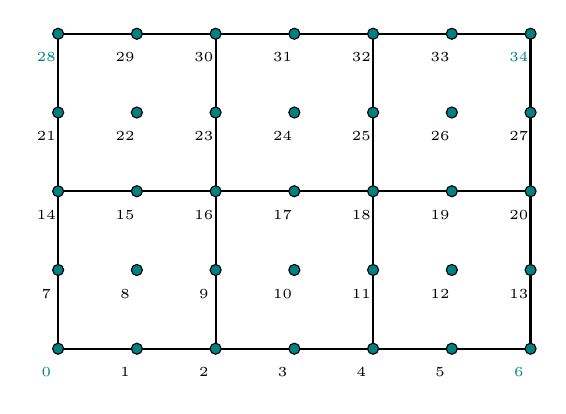
\begin{tikzpicture}
%\draw[step=0.5cm,gray,very thin] (0,0) grid (8,6); %background grid

\draw[thick] (1,1) -- (7,1) -- (7,5) -- (1,5) -- cycle;  
\draw[thick] (1,3) -- (7,3) ;
\draw[thick] (3,1) -- (3,5) ;
\draw[thick] (5,1) -- (5,5) ;

\draw[black,fill=teal] (1,1)     circle (2pt); 
\draw[black,fill=teal] (2,1)     circle (2pt); 
\draw[black,fill=teal] (3,1)     circle (2pt); 
\draw[black,fill=teal] (4,1)     circle (2pt); 
\draw[black,fill=teal] (5,1)     circle (2pt); 
\draw[black,fill=teal] (6,1)     circle (2pt); 
\draw[black,fill=teal] (7,1)     circle (2pt); 

\draw[black,fill=teal] (1,2)     circle (2pt); 
\draw[black,fill=teal] (2,2)     circle (2pt); 
\draw[black,fill=teal] (3,2)     circle (2pt); 
\draw[black,fill=teal] (4,2)     circle (2pt); 
\draw[black,fill=teal] (5,2)     circle (2pt); 
\draw[black,fill=teal] (6,2)     circle (2pt); 
\draw[black,fill=teal] (7,2)     circle (2pt); 

\draw[black,fill=teal] (1,3)     circle (2pt); 
\draw[black,fill=teal] (2,3)     circle (2pt); 
\draw[black,fill=teal] (3,3)     circle (2pt); 
\draw[black,fill=teal] (4,3)     circle (2pt); 
\draw[black,fill=teal] (5,3)     circle (2pt); 
\draw[black,fill=teal] (6,3)     circle (2pt); 
\draw[black,fill=teal] (7,3)     circle (2pt); 

\draw[black,fill=teal] (1,4)     circle (2pt); 
\draw[black,fill=teal] (2,4)     circle (2pt); 
\draw[black,fill=teal] (3,4)     circle (2pt); 
\draw[black,fill=teal] (4,4)     circle (2pt); 
\draw[black,fill=teal] (5,4)     circle (2pt); 
\draw[black,fill=teal] (6,4)     circle (2pt); 
\draw[black,fill=teal] (7,4)     circle (2pt); 

\draw[black,fill=teal] (1,5)     circle (2pt); 
\draw[black,fill=teal] (2,5)     circle (2pt); 
\draw[black,fill=teal] (3,5)     circle (2pt); 
\draw[black,fill=teal] (4,5)     circle (2pt); 
\draw[black,fill=teal] (5,5)     circle (2pt); 
\draw[black,fill=teal] (6,5)     circle (2pt); 
\draw[black,fill=teal] (7,5)     circle (2pt); 

\node[] at (0.85,0.7) {\tiny \color{teal} 0};
\node[] at (1.85,0.7) {\tiny 1};
\node[] at (2.85,0.7) {\tiny 2};
\node[] at (3.85,0.7) {\tiny 3};
\node[] at (4.85,0.7) {\tiny 4};
\node[] at (5.85,0.7) {\tiny 5};
\node[] at (6.85,0.7) {\tiny \color{teal} 6};

\node[] at (0.85,1.7) {\tiny 7};
\node[] at (1.85,1.7) {\tiny 8};
\node[] at (2.85,1.7) {\tiny 9};
\node[] at (3.85,1.7) {\tiny 10};
\node[] at (4.85,1.7) {\tiny 11};
\node[] at (5.85,1.7) {\tiny 12};
\node[] at (6.85,1.7) {\tiny 13};

\node[] at (0.85,2.7) {\tiny 14}; 
\node[] at (1.85,2.7) {\tiny 15}; 
\node[] at (2.85,2.7) {\tiny 16}; 
\node[] at (3.85,2.7) {\tiny 17}; 
\node[] at (4.85,2.7) {\tiny 18}; 
\node[] at (5.85,2.7) {\tiny 19}; 
\node[] at (6.85,2.7) {\tiny 20}; 

\node[] at (0.85,3.7) {\tiny 21}; 
\node[] at (1.85,3.7) {\tiny 22}; 
\node[] at (2.85,3.7) {\tiny 23}; 
\node[] at (3.85,3.7) {\tiny 24}; 
\node[] at (4.85,3.7) {\tiny 25}; 
\node[] at (5.85,3.7) {\tiny 26}; 
\node[] at (6.85,3.7) {\tiny 27}; 

\node[] at (0.85,4.7) {\tiny \color{teal} 28}; 
\node[] at (1.85,4.7) {\tiny 29}; 
\node[] at (2.85,4.7) {\tiny 30}; 
\node[] at (3.85,4.7) {\tiny 31}; 
\node[] at (4.85,4.7) {\tiny 32}; 
\node[] at (5.85,4.7) {\tiny 33}; 
\node[] at (6.85,4.7) {\tiny \color{teal} 34}; 

\end{tikzpicture}


\end{center}

Concretely here:
\begin{itemize}
\item nodes {\color{teal} 0,6,28,34} see 9 nodes (corners)
\item nodes 1,3,5,7,8,10,12,13,21,22,24,26,27,29,31,33 see 9 nodes
\item nodes 2,4,9,11,14,15,17,19,20,23,25,30,32, see 15 nodes
\item nodes 16,18 see 25 nodes
\end{itemize}

If there was only one dof per node, we would find 
the number of non zeros as follow:
\[
NZ=4*9 + 16*9 + 13*15 + 2*25 = 36+144 + 195 + 50 = 425
\]
But since there are two velocity dofs per node, we find that 
the total number of nonzeros is 4 times higher, i.e.
\[
NZ=1700
\] 
And if we choose for a symmetric CSR storage:
\[
NZ_{symm} = \frac{NZ-N}{2}+N = \frac{1700-70}{2} + 70 = 885 
\]

Let us now turn to the real case of 2 dofs per node and establish who 'sees' who:

\begin{tabular}{lp{14.5cm}l}
dof &  sees other dofs & total\\
\hline
0 & 0,1,2,3,4,5,14,15,16,17,18,19,28,29,30,31,32,33 & 18 \\
1 & 0,1,2,3,4,5,14,15,16,17,18,19,28,29,30,31,32,33 & 18 \\
2 & 0,1,2,3,4,5,14,15,16,17,18,19,28,29,30,31,32,33 & 18 \\
3 & 0,1,2,3,4,5,14,15,16,17,18,19,28,29,30,31,32,33 & 18 \\
4 & 0,1,2,3,4,5,6,7,8,9,14,15,16,17,18,19,20,21,22,23,28,29,30,31,32,33,34,35,36,37 & 30 \\
5 & 0,1,2,3,4,5,6,7,8,9,14,15,16,17,18,19,20,21,22,23,28,29,30,31,32,33,34,35,36,37 & 30 \\
6 & 4,5,6,7,8,9,18,19,20,21,22,23,32,33,34,35,36,37 & 18 \\
7 & 4,5,6,7,8,9,18,19,20,21,22,23,32,33,34,35,36,37 & 18 \\
8 & 4,5,6,7,8,9,10,11,12,13,18,19,20,21,22,23,24,25,26,27,32,33,34,35,36,37,38,39,40,41 & 30 \\
9 & 4,5,6,7,8,9,10,11,12,13,18,19,20,21,22,23,24,25,26,27,32,33,34,35,36,37,38,39,40,41 & 30 \\
10 & 8,9,10,11,12,13,22,23,24,25,26,27,36,37,38,39,40,41 & 18\\
11 & 8,9,10,11,12,13,22,23,24,25,26,27,36,37,38,39,40,41 & 18\\
12 & 8,9,10,11,12,13,22,23,24,25,26,27,36,37,38,39,40,41 & 18\\
13 & 8,9,10,11,12,13,22,23,24,25,26,27,36,37,38,39,40,41 & 18\\
14 & 0,1,2,3,4,5,14,15,16,17,18,19,28,29,30,31,32,33 & 18 \\
15 & 0,1,2,3,4,5,14,15,16,17,18,19,28,29,30,31,32,33 & 18 \\
16 & 0,1,2,3,4,5,14,15,16,17,18,19,28,29,30,31,32,33 & 18 \\
17 & 0,1,2,3,4,5,14,15,16,17,18,19,28,29,30,31,32,33 & 18 \\
 ... & ... & ... \\
68 & 36,37,38,39,50,51,52,53,54,55,64,65,66,67,68,69 & 18 \\
69 & 36,37,38,39,50,51,52,53,54,55,64,65,66,67,68,69 & 18 \\
\hline
\end{tabular}

The second column of this array is the content of the {\sffamily ja} array 
if a full storage is used.
If we now use a symmetric storage then:

\begin{tabular}{lp{14.5cm}l}
dof &  sees other dofs & total\\
\hline
0 & 0,1,2,3,4,5,14,15,16,17,18,19,28,29,30,31,32,33 & 18 \\
1 & 1,2,3,4,5,14,15,16,17,18,19,28,29,30,31,32,33 & 17 \\
2 & 2,3,4,5,14,15,16,17,18,19,28,29,30,31,32,33 & 16 \\
3 & 3,4,5,14,15,16,17,18,19,28,29,30,31,32,33 & 15 \\
4 & 4,5,6,7,8,9,14,15,16,17,18,19,20,21,22,23,28,29,30,31,32,33,34,35,36,37 &  \\
5 & 5,6,7,8,9,14,15,16,17,18,19,20,21,22,23,28,29,30,31,32,33,34,35,36,37 &  \\
6 & 6,7,8,9,18,19,20,21,22,23,32,33,34,35,36,37 &  \\
7 & 7,8,9,18,19,20,21,22,23,32,33,34,35,36,37 &  \\
8 & 8,9,10,11,12,13,18,19,20,21,22,23,24,25,26,27,32,33,34,35,36,37,38,39,40,41 &  \\
9 & 9,10,11,12,13,18,19,20,21,22,23,24,25,26,27,32,33,34,35,36,37,38,39,40,41 &  \\
10 & 10,11,12,13,22,23,24,25,26,27,36,37,38,39,40,41 & \\
11 & 11,12,13,22,23,24,25,26,27,36,37,38,39,40,41 & \\
12 & 12,13,22,23,24,25,26,27,36,37,38,39,40,41 & \\
13 & 13,22,23,24,25,26,27,36,37,38,39,40,41 & \\
14 & 14,15,16,17,18,19,28,29,30,31,32,33 &  \\
15 & 15,16,17,18,19,28,29,30,31,32,33 &  \\
16 & 16,17,18,19,28,29,30,31,32,33 &  \\
17 & 17,18,19,28,29,30,31,32,33 &  \\
 ... & ... & ... \\
68 & 68,69 & 2 \\
69 & 69 & 1 \\
\hline
\end{tabular}









In order establish a pattern we will need a bigger mesh:

\begin{center}
\begin{flushright} {\footnotesize {\color{gray} (tikz\_4x3\_Q2.tex)}} \end{flushright}
%~~~~~~~~~~~~~~~~~~~~~~~~~~~~~~~~~~~~~~~~~~~~~~~~~~~~~~~~~~~~~~~~~~~~~~~~~~~~~~~~~~~~~~~~~~~~~~~~~~

\begin{tikzpicture}
%\draw[step=0.5cm,gray,very thin] (0,0) grid (10,8); %background grid

\draw[thick] (1,1) -- (9,1) -- (9,7) -- (1,7) -- cycle;  
\draw[thick] (1,3) -- (9,3) ;
\draw[thick] (1,5) -- (9,5) ;
\draw[thick] (3,1) -- (3,7) ;
\draw[thick] (5,1) -- (5,7) ;
\draw[thick] (7,1) -- (7,7) ;

\draw[black,fill=teal] (1,1)     circle (2pt);  %0
\draw[black,fill=violet] (2,1)     circle (2pt); 
\draw[black,fill=chestnut] (3,1)     circle (2pt); 
\draw[black,fill=violet] (4,1)     circle (2pt); 
\draw[black,fill=chestnut] (5,1)     circle (2pt); 
\draw[black,fill=violet] (6,1)     circle (2pt); 
\draw[black,fill=chestnut] (7,1)     circle (2pt); 
\draw[black,fill=violet] (8,1)     circle (2pt); 
\draw[black,fill=teal] (9,1)     circle (2pt); %8

\draw[black,fill=violet] (1,2)     circle (2pt); %9
\draw[black,fill=green] (2,2)     circle (2pt); 
\draw[black,fill=carrotorange] (3,2)     circle (2pt); 
\draw[black,fill=green] (4,2)     circle (2pt); 
\draw[black,fill=carrotorange] (5,2)     circle (2pt); 
\draw[black,fill=green] (6,2)     circle (2pt); 
\draw[black,fill=carrotorange] (7,2)     circle (2pt); 
\draw[black,fill=green] (8,2)     circle (2pt); 
\draw[black,fill=violet] (9,2)     circle (2pt); %17

\draw[black,fill=chestnut] (1,3)     circle (2pt); %18
\draw[black,fill=carrotorange] (2,3)     circle (2pt); 
\draw[black,fill=blue] (3,3)     circle (2pt); 
\draw[black,fill=carrotorange] (4,3)     circle (2pt); 
\draw[black,fill=blue] (5,3)     circle (2pt); 
\draw[black,fill=carrotorange] (6,3)     circle (2pt); 
\draw[black,fill=blue] (7,3)     circle (2pt); 
\draw[black,fill=carrotorange] (8,3)     circle (2pt); 
\draw[black,fill=chestnut] (9,3)     circle (2pt); %26

\draw[black,fill=violet] (1,4)     circle (2pt); %27
\draw[black,fill=green] (2,4)     circle (2pt); 
\draw[black,fill=carrotorange] (3,4)     circle (2pt); 
\draw[black,fill=green] (4,4)     circle (2pt); 
\draw[black,fill=carrotorange] (5,4)     circle (2pt); 
\draw[black,fill=green] (6,4)     circle (2pt); 
\draw[black,fill=carrotorange] (7,4)     circle (2pt); 
\draw[black,fill=green] (8,4)     circle (2pt); 
\draw[black,fill=violet] (9,4)     circle (2pt); %35

\draw[black,fill=chestnut] (1,5)     circle (2pt); %36
\draw[black,fill=carrotorange] (2,5)     circle (2pt); 
\draw[black,fill=blue] (3,5)     circle (2pt); 
\draw[black,fill=carrotorange] (4,5)     circle (2pt); 
\draw[black,fill=blue] (5,5)     circle (2pt); 
\draw[black,fill=carrotorange] (6,5)     circle (2pt); 
\draw[black,fill=blue] (7,5)     circle (2pt); 
\draw[black,fill=carrotorange] (8,5)     circle (2pt); 
\draw[black,fill=chestnut] (9,5)     circle (2pt); %44

\draw[black,fill=violet] (1,6)     circle (2pt); %45 
\draw[black,fill=green] (2,6)     circle (2pt); 
\draw[black,fill=carrotorange] (3,6)     circle (2pt); 
\draw[black,fill=green] (4,6)     circle (2pt); 
\draw[black,fill=carrotorange] (5,6)     circle (2pt); 
\draw[black,fill=green] (6,6)     circle (2pt); 
\draw[black,fill=carrotorange] (7,6)     circle (2pt); 
\draw[black,fill=green] (8,6)     circle (2pt); 
\draw[black,fill=violet] (9,6)     circle (2pt); %53

\draw[black,fill=teal] (1,7)     circle (2pt); %54
\draw[black,fill=violet] (2,7)     circle (2pt); 
\draw[black,fill=chestnut] (3,7)     circle (2pt); 
\draw[black,fill=violet] (4,7)     circle (2pt); 
\draw[black,fill=chestnut] (5,7)     circle (2pt); 
\draw[black,fill=violet] (6,7)     circle (2pt); 
\draw[black,fill=chestnut] (7,7)     circle (2pt); 
\draw[black,fill=violet] (8,7)     circle (2pt); 
\draw[black,fill=teal] (9,7)     circle (2pt); %62

\node[] at (0.825,0.7) {\footnotesize \color{teal} 0};
\node[] at (1.825,0.7) {\footnotesize \color{violet} 1};
\node[] at (2.825,0.7) {\footnotesize \color{chestnut} 2};
\node[] at (3.825,0.7) {\footnotesize \color{violet} 3};
\node[] at (4.825,0.7) {\footnotesize \color{chestnut} 4};
\node[] at (5.825,0.7) {\footnotesize \color{violet} 5};
\node[] at (6.825,0.7) {\footnotesize \color{chestnut} 6};
\node[] at (7.825,0.7) {\footnotesize \color{violet} 7};
\node[] at (8.825,0.7) {\footnotesize \color{teal} 8};

\node[] at (0.825,1.7) {\footnotesize \color{violet} 9};
\node[] at (1.825,1.7) {\footnotesize \color{green} 10};
\node[] at (2.825,1.7) {\footnotesize \color{carrotorange}11};
\node[] at (3.825,1.7) {\footnotesize \color{green} 12};
\node[] at (4.825,1.7) {\footnotesize \color{carrotorange}13};
\node[] at (5.825,1.7) {\footnotesize \color{green} 14};
\node[] at (6.825,1.7) {\footnotesize \color{carrotorange}15};
\node[] at (7.825,1.7) {\footnotesize \color{green} 16};
\node[] at (8.825,1.7) {\footnotesize \color{violet} 17};

\node[] at (0.825,2.7) {\footnotesize \color{chestnut} 18}; 
\node[] at (1.825,2.7) {\footnotesize \color{carrotorange} 19}; 
\node[] at (2.825,2.7) {\footnotesize \color{blue} 20}; 
\node[] at (3.825,2.7) {\footnotesize \color{carrotorange} 21}; 
\node[] at (4.825,2.7) {\footnotesize \color{blue} 22}; 
\node[] at (5.825,2.7) {\footnotesize \color{carrotorange} 23}; 
\node[] at (6.825,2.7) {\footnotesize \color{blue} 24}; 
\node[] at (7.825,2.7) {\footnotesize \color{carrotorange} 25}; 
\node[] at (8.825,2.7) {\footnotesize \color{chestnut} 26}; 

\node[] at (0.825,3.7) {\footnotesize \color{violet} 27}; 
\node[] at (1.825,3.7) {\footnotesize \color{green} 28}; 
\node[] at (2.825,3.7) {\footnotesize \color{carrotorange} 29}; 
\node[] at (3.825,3.7) {\footnotesize \color{green} 30}; 
\node[] at (4.825,3.7) {\footnotesize \color{carrotorange} 31}; 
\node[] at (5.825,3.7) {\footnotesize \color{green} 32}; 
\node[] at (6.825,3.7) {\footnotesize \color{carrotorange} 33}; 
\node[] at (7.825,3.7) {\footnotesize \color{green} 34}; 
\node[] at (8.825,3.7) {\footnotesize \color{violet} 35};

\node[] at (0.825,4.7) {\footnotesize \color{chestnut} 36}; 
\node[] at (1.825,4.7) {\footnotesize \color{carrotorange}37}; 
\node[] at (2.825,4.7) {\footnotesize \color{blue} 38}; 
\node[] at (3.825,4.7) {\footnotesize \color{carrotorange}39}; 
\node[] at (4.825,4.7) {\footnotesize \color{blue} 40}; 
\node[] at (5.825,4.7) {\footnotesize \color{carrotorange}41}; 
\node[] at (6.825,4.7) {\footnotesize \color{blue} 42};
\node[] at (7.825,4.7) {\footnotesize \color{carrotorange}43};
\node[] at (8.825,4.7) {\footnotesize \color{chestnut} 44};

\node[] at (0.825,5.7) {\footnotesize \color{violet} 45}; 
\node[] at (1.825,5.7) {\footnotesize \color{green} 46}; 
\node[] at (2.825,5.7) {\footnotesize \color{carrotorange}47}; 
\node[] at (3.825,5.7) {\footnotesize \color{green} 48}; 
\node[] at (4.825,5.7) {\footnotesize \color{carrotorange}49}; 
\node[] at (5.825,5.7) {\footnotesize \color{green} 50}; 
\node[] at (6.825,5.7) {\footnotesize \color{carrotorange}51};
\node[] at (7.825,5.7) {\footnotesize \color{green} 52};
\node[] at (8.825,5.7) {\footnotesize \color{violet} 53};

\node[] at (0.825,6.7) {\footnotesize \color{teal}54}; 
\node[] at (1.825,6.7) {\footnotesize \color{violet} 55}; 
\node[] at (2.825,6.7) {\footnotesize \color{chestnut} 56}; 
\node[] at (3.825,6.7) {\footnotesize \color{violet} 57}; 
\node[] at (4.825,6.7) {\footnotesize \color{chestnut} 58}; 
\node[] at (5.825,6.7) {\footnotesize \color{violet} 59}; 
\node[] at (6.825,6.7) {\footnotesize \color{chestnut} 60};
\node[] at (7.825,6.7) {\footnotesize \color{violet} 61};
\node[] at (8.825,6.7) {\footnotesize \color{teal} 62};

\end{tikzpicture}

\end{center}



We have
\begin{itemize}
\item {\color{teal} 4} corner nodes which have 9 neighbours
\item {\color{green} $nel$} mid-element nodes which have 9 neighbours
\item {\color{violet} $2*nelx+2*nely$} mid-edge nodes on sides which have 9 neighbours
\item {\color{carrotorange} $(nelx-1)*nely+nelx*(nely-1)$} internal mid-edges nodes which have 15 neighbours
\item {\color{chestnut} $2*(nelx-1)+2*(nely-1)$} side nodes that have 15 neighbours 
\item {\color{blue} $(nelx-1)*(nely-1)$} nodes which have 25 neighbours
\end{itemize}
In the end, the number of non-zeros ($Q_1$) is given by
\begin{eqnarray}
NZ 
&=& {\color{teal} 4 }*9 \nn\\
&+& {\color{green} nel }*9 \nn\\
&+& {\color{violet} (2*nelx+2*nely) }*9 \nn\\
&+& {\color{carrotorange} [(nelx-1)*nely+nelx*(nely-1)] }*15 \nn\\
&+& {\color{chestnut} [2*(nelx-1)+2*(nely-1)] }*15 \nn\\
&+& {\color{blue} (nelx-1)*(nely-1) }*25 \nn
\end{eqnarray}
Verification: $nelx=3$, $nely=2$:
\begin{eqnarray}
NZ
&=& 4*9 + 6*9 + (2*3+2*2)*9 + [(3-1)*2+3*(2-1)]*15
+ [2*(3-1)+2*(2-1)]*15 + (3-1)*(2-1)*25 \nn\\
&=& 36 + 54 + 10*9 + 7*15 + 6*15 + 2*25 \nn\\
&=& 36 + 54 + 90 + 105 + 90 + 50  \nn\\
&=& 425 \nn
\end{eqnarray}
as expected.








%..............................................................................
\subsection{3d domain - $Q_1$ - CSR storage - One degree of freedom}

Let us consider a $3\times4\times2$ grid which counts 
$nnx\cdot nny \cdot nnz = 5 \cdot 4\cdot 3=60$ nodes.
The assembled FEM matrix $\K$ size is then 
$N=nnx\times nny\times nnz \times ndof=180$.

\begin{center}
\input{tikz/tikz_4x3x2.tex}
\end{center}



The total number of nonzeros in the case $ndof=1$ would be decomposed as follows:
\begin{itemize}
\item 8 corners 'see' 8 neighbours
\item 4 edges with $(nnx-2)$ nodes in the x direction see 12 nodes
\item 4 edges with $(nny-2)$ nodes in the y direction see 12 nodes
\item 4 edges with $(nnz-2)$ nodes in the z direction see 12 nodes
\item $2(nnx-2)(nny-2)$ nodes see 18 nodes
\item $2(nnx-2)(nnz-2)$ nodes see 18 nodes
\item $2(nny-2)(nnz-2)$ nodes see 18 nodes
\item $(nnx-2)(nny-2)(nnz-2)$ interior nodes see 27 nodes
\end{itemize}

%..............................................................................
\subsection{3d domain - $Q_2$ - CSR storage - one degree of freedom}


\begin{center}
\input{tikz/tikz_4x3x2_q2.tex}
\end{center}





%..............................................................................
\subsection{Matrix Storage in the Python codes of FieldStone}

The majority of the early codes have the FE matrix being a full array
\begin{lstlisting}
a_mat = np.zeros((Nfem,Nfem),dtype=np.float64) 
\end{lstlisting}
and it is converted to CSR format on the fly in the solve phase:
\begin{lstlisting}
sol = sps.linalg.spsolve(sps.csr_matrix(a_mat),rhs)
\end{lstlisting}

Note that linked list storages can be used (lil\_matrix). Substantial memory savings 
but much longer compute times since it takes longer to write in such arrays.
A conversion to CSR format is still necessary before calling the solver.




%..............................................................................
\subsection{About Sparse Matrix-Vector multiplication} \label{ss:spmv}
\index{general}{SpMV} \index{general}{Sparse Matrix-Vector Multiplication}

When the matrix ${\bm A}$ is stored in a two-dimensional array of size $N\times N$, 
its (left or right) multiplication by a vector is trivial. 
Either one resorts to writing a double for loop (not recommended), 
either one uses {\tt numpy.dot}\footnote{\url{https://numpy.org/doc/stable/reference/generated/numpy.dot.html}}
in python, or {\tt matmul} in Fortran.

However, when the matrix is stored as a single continuous array, say CSR, how does this work?
This question is {\it very important} since iterative solvers such as the Conjugate Gradient solver
(see Section~\ref{ss:itsolvers}) rely extensively on multiplying the matrix by many different vectors. 

The Sparse Matrix-Vector multiplication operation is often abbreviated SpMV.
To quote Knepley \cite{knepley}: "The Sparse Matrix-Vector Product (SpMV) is today 
a workhorse of scientific computing. It is a central kernel in iterative linear and 
nonlinear solvers for PDE, and now for many graph algorithms."
As explained in Williams \etal (2007) \cite{wiov07} (and in many 
other sources on the topic), the algorithm for 
a basic SpMV implementation is rather simple in its naive form: 

\begin{center}
\includegraphics[width=17cm]{images/spmv/widc08}\\
{\captionfont Taken from Williams \etal (2008) \cite{widc08}. 
Sparse Matrix Vector Multiplication (SpMV). 
(a) visualization of the algebra: $\vec{y} \leftarrow {\bm A}\cdot \vec{x}$.
(b) Standard compressed sparse row (CSR) representation of the matrix.
(c) The standard implementation of SpMV for a matrix stored in CSR. 
The outer loop is trivially parallelized without any data dependencies.}
\end{center}

Let us assume that we wish to compute $\vec{y}={\bm A}\cdot \vec{x}$ where ${\bm A}$ 
is in CSR format. The pseudo code then goes as follows:
\begin{lstlisting}
for i in range(0,m):
    y0=0
    for k in range(ROWPTR[i],ROWPTR[i+1]):
        y0 += VAL[k] * x[COLIND[k]]
    y[i]=y0
\end{lstlisting} 
Although technically correct, this algorithm is problematic because the vector x array
is accessed indirectly and this causes a non-optimal use of the processor, which 
in the end makes the calculation take longer than it should.


The following piece of ForTran code comes from \elefant. 
Note that here (ROWPTR=ia, COLIND=ja, VAL=mat)
\begin{lstlisting}[language=Fortran]
subroutine spmv (nr,nc,nz,x,y,mat,ja,ia)
implicit none
integer, intent(in)  :: nr,nc,nz
real(8), intent(in)  :: x(nc), mat(nz)
real(8), intent(out) :: y(nr)
integer, intent(in)  :: ja(nz),ia(nr+1)
real(8) t
integer i, k

do i = 1,nr
   t = 0.0d0
   do k=ia(i), ia(i+1)-1
      t = t + mat(k)*x(ja(k))
   end do
   y(i) = t 
end do

end subroutine
\end{lstlisting}


How to make this calculation as efficiently as possible on CPUs and GPUs, on one thread 
or multiple threads has given rise to a lot of literature.

\Literature: 
\textcite{krda10} (2010), Section 9.4 of \textcite{knepley}, 
\textcite{widc08} (2008).

%..............................................................................
\subsection{SpMV and SpMV-T with the CSR format - a concrete example}

(What follows was orignally written for \elefant so that code excerpts and loop indexing 
are those of Fortran.)

Let us consider a simple matrix $\mathbb{G}$ which is not square (size is $3\times5$):
\[
\G^T=
\left(
\begin{array}{ccccc}
{\color{teal} 1} & {\color{teal}0}& {\color{teal}4}& {\color{teal}1}& {\color{teal}2}\\
{\color{violet}0}& {\color{violet}1}& {\color{violet}1}& {\color{violet}1}& {\color{violet}0}\\
{\color{orange}3}& {\color{orange}0} & {\color{orange}0}& {\color{orange}7}& {\color{orange}1}
\end{array}
\right)
\]

The number of rows is $nr=3$, the number of columns is $nc=5$ and the number of nonzeros is 
$nz=10$.

Let us consider two vectors $\vec{\cal V}^T=(1,1,1,1,1)$ and $\vec{\cal P}^T=(1,1,1)$.
Obviously, we have:
\[
{\G}^T \cdot \vec{\cal V} = 
\left(
\begin{array}{c}
8\\3\\11
\end{array}
\right)
\qquad
\text{and}
\qquad
{\G} \cdot \vec{\cal P} = 
\left(
\begin{array}{c}
4 \\ 1\\ 5\\ 9\\ 3
\end{array}
\right)
\]

The CSR storage of ${\G}^T$ requires three arrays:
$ia$ (integer, size $nr+1$), $ja$ (integer, size $nz$) and $mat$ (real, size $nz$). 
In the case of the small matrix above:
\begin{eqnarray}
ia &=&(1,5,8,11)  \nn\\
ja &=&(1,3,4,5,2,3,4,1,4,5) \nn\\
mat&=&({\color{teal} 1,4,1,2},{\color{violet}1,1,1},{\color{orange}3,7,1}) \nn
\end{eqnarray}
The sparse matrix vector multiplication kernel SpMV for $\vec{y} = {\bm A}\cdot \vec{x}$ 
has been explained above, and it is trivial to carry out this algorithm by hand 
and verify that the vector $y$ is given by $y^T=(8,3,11)$.

Let us now turn to an interesting problem. Is it possible with the same arrays $ia,ja,mat$ to compute the 
multiplication of the transpose of the matrix with a vector? 
The answer is of course positive and the code is given hereunder:

\begin{lstlisting}[language=Fortran]
y=0.d0
do i = 1,nr
   do k=ia(i), ia(i+1)-1
      y(ja(k))=y(ja(k))+mat(k)*x(i)
   end do
end do
\end{lstlisting}

Let us take $i=1$. The variable $k$ then goes from 1 to 4. 
The inner loop does:
\begin{verbatim}
y(1)=y(1)+mat(1)*x(1)
y(3)=y(3)+mat(2)*x(1)
y(4)=y(4)+mat(3)*x(1)
y(5)=y(5)+mat(4)*x(1)
\end{verbatim}

Let us take $i=2$. The variable $k$ then goes from 5 to 7. 
The inner loop does:
\begin{verbatim}
y(2)=y(2)+mat(5)*x(2)
y(3)=y(3)+mat(6)*x(2)
y(4)=y(4)+mat(7)*x(2)
\end{verbatim}

Let us take $i=3$. The variable $k$ then goes from 8 to 10. 
The inner loop does:
\begin{verbatim}
y(1)=y(1)+mat(8)*x(3)
y(4)=y(4)+mat(9)*x(3)
y(5)=y(5)+mat(10)*x(3)
\end{verbatim}

So in total, we have:
\begin{verbatim}
y(1)=mat(1)*x(1)+mat(8)*x(3)
y(2)=mat(5)*x(2)
y(3)=mat(2)*x(1)+mat(6)*x(2)
y(4)=mat(3)*x(1)+mat(7)*x(2)+mat(9)*x(3)
y(5)=mat(4)*x(1)+mat(10)*x(3)
\end{verbatim}
which is indeed the result of the transposed of the matrix multiplied by a vector $\vec{x}$.

\vspace{0.6cm}

Let us consider a simple matrix $\K$ which is square (size is $5\times5$):
\[
\K=
\left(
\begin{array}{ccccc}
1&0&4&1&2\\
0&1&0&1&0\\
4&0&0&7&1\\
1&1&7&4&0\\
2&0&1&0&5
\end{array}
\right)
\]

In this case , NZ=16.
\begin{eqnarray}
ia &=&(1,5,7,10,14,17) \nn\\
ja &=&(1,3,4,5,\;\; 2,4, \;\; 1,4,5, \;\; 1,2,3,4, \;\; 1,3,5) \nn\\
mat&=&(1,4,1,2,1,1,4,7,1,1,1,7,4,2,1,5) \nn
\end{eqnarray}
The sparse matrix vector multiplication kernel SpMV for $\vec{y} = {\bm A}\cdot \vec{x}$ 
is given  as follows in its simplest form.
Since the matrix is symmetric, there is no use to store the whole matrix. Its upper half (for instance) will do. 
In this case, NZ=
and then 
\begin{eqnarray}
ia &=&(1,5,7,9,10,11) \nn\\
ja &=&(1,3,4,5,\;\; 2,4, \;\; 4,5, \;\; 4, \;\; 5) \nn\\
mat&=&(1,4,1,2,\;\; 1,1, \;\; 7,1, \;\; 4,\;\; 5) \nn
\end{eqnarray}

All is good and well until one wishes to multiply the real matrix by a vector. 
The SpMV routines described above will not work since it will return the upper half of the matrix 
multiplied by the vector.

One can then write a decicated algorithm:
\begin{verbatim}
do i = 1,nr

   ! multiply the upper half by the vector

   do k=ia(i), ia(i+1)-1
      y(i) = y(i) + mat(k)*x(ja(k))
   end do

   ! multiply the transpose of matrix by vector
   ! but omit diagonal 

   do k=ia(i), ia(i+1)-1
      if (i/=ja(k)) then
         y(ja(k))=y(ja(k))+mat(k)*x(i)
      end if
   end do

end do
\end{verbatim}


Example:

\begin{verbatim}
y(1)
=y(1) + mat(1)*x(ja(1)) + mat(2)*x(ja(2)) + mat(3)*x(ja(3)) + mat(4)*x(ja(4)) 
=y(1) + mat(1)*x(1) + mat(2)*x(3) + mat(3)*x(4) + mat(4)*x(5) 
\end{verbatim}
etc ...

Finish?

 




